% Lean-certified smoothed optimization core for the DK journal paper.
\section{Exact smoothed spectral transport}
\label{sec:smoothed-transport}

The counterexample to Proposition~4.4 leaves a norm-dependent question:
which displacement penalties favor the direct rotation, and what replaces
it when they do not? We answer this question exactly for a smooth
singular-value penalty on finite-dimensional complex spaces. The answer
includes a transition angle, a globally minimizing unitary, and a bound on
the distance of every near-minimizer from the canonical rotation below
the transition.

Throughout this section $U,V\subseteq\mathbb C^n$ have equal dimension
$r$, with orthogonal projections $P,Q$ and principal angles
$\theta_1,\ldots,\theta_r\in[0,\pi/2]$.

For $\tau>0$, define the smooth spectral displacement cost
\[
 \Psi_\tau(W)=\operatorname{tr}
  \sqrt{\tau^2I+(I-W)^*(I-W)}-n\tau.
\]
Each displacement singular value $s$ contributes
$\rho_\tau(s)=\sqrt{\tau^2+s^2}-\tau$. This penalty is quadratic near
zero and asymptotically linear. Hyperbolic singular-value penalties of
this form, up to a positive scale and an additive constant, are used in
low-rank inverse-problem regularization \citep{lobos2026smooth}. Put
\[
 \eta=\frac{\tau+\sqrt{\tau^2+4}}2>1,
 \qquad c_\tau=\arccos(\eta^{-2}).
\]
The identity $\tau=\eta-\eta^{-1}$ gives, for every unitary $W$,
\begin{equation}
 \Psi_\tau(W)=\|\eta W-\eta^{-1}I\|_1-n\tau.
 \label{eq:smoothed-weighted-nuclear}
\end{equation}
Indeed, both positive square roots are applied to the same matrix,
namely $(\tau^2+2)I-W-W^*$.

\begin{theorem}[Exact smoothed transport]
\label{thm:smoothed-transport}
For the subspaces and smoothing parameter above,
\begin{equation}
 \min_{WPW^*=Q}\Psi_\tau(W)=\sum_{j=1}^r \mu_\tau(\theta_j),
 \label{eq:smoothed-global-minimum}
\end{equation}
where the minimum is over unitary $W$ and
\[
 \mu_\tau(\theta)=
 \begin{cases}
  2\bigl(\sqrt{\tau^2+2-2\cos\theta}-\tau\bigr),
        &0\leq\theta\leq c_\tau,\\
  2\eta\sin\theta-2\tau,
        &c_\tau\leq\theta\leq\pi/2.
 \end{cases}
\]
An attaining transporter is the identity on the fixed summands of a
cosine--sine decomposition and $e^{i\delta_\tau(\theta)}R_\theta$ on
each nonzero principal plane, where
\[
 R_\theta=\begin{pmatrix}\cos\theta&-\sin\theta\\
                              \sin\theta&\cos\theta\end{pmatrix},
 \qquad
 \delta_\tau(\theta)=
 \begin{cases}
   0,&\theta\leq c_\tau,\\
   \arccos(\eta^2\cos\theta),&\theta\geq c_\tau.
 \end{cases}
\]
Either sign of the displayed phase gives an attaining transporter.
The nonnegative choice uniquely minimizes the scalar-phase cost over
$[0,\theta]$.
\end{theorem}

\begin{lstlisting}[style=leanpaper,
 caption={Lean signature for the unrestricted minimum. The surrounding
 finite-dimensional complex Hilbert-space context is omitted.
 \texttt{smoothedDisplacementCost} is $\Psi_\tau$ and
 \texttt{smoothedPhaseMinimum} is $\mu_\tau$.
 The conclusion gives an attaining unitary and the lower bound for
 every admissible competitor.},
 label={lst:smoothed-global}]
theorem exists_unitary_minimizing_smoothed_transport_principalAngles
    (tau : Real) (htau : 0 < tau) (U V : Submodule Complex E)
    (hUV : Module.finrank Complex U = Module.finrank Complex V) :
    ∃ W : LinearIsometryEquiv (RingHom.id Complex) E E,
      U.map W.toLinearMap = V ∧
      smoothedDisplacementCost tau W.toLinearMap =
        (Finset.univ.sum (fun i : Fin (Module.finrank Complex U) =>
          smoothedPhaseMinimum tau (U.principalAngles V i))) ∧
      ∀ T : LinearIsometryEquiv (RingHom.id Complex) E E,
        U.map T.toLinearMap = V ->
        (Finset.univ.sum (fun i : Fin (Module.finrank Complex U) =>
          smoothedPhaseMinimum tau (U.principalAngles V i))) <=
            smoothedDisplacementCost tau T.toLinearMap
\end{lstlisting}

\begin{proof}
We first prove the scalar claim. Write $a=\eta$, $b=\eta^{-1}$, and
use an auxiliary complex plane. The scalar cost plus
$2\tau$ is the sum of the distances from $x=be^{i\delta}$ to the two
points $u=ae^{i\theta}$ and $v=ae^{-i\theta}$:
\begin{equation}
 \rho_\tau\bigl(2\sin((\theta+\delta)/2)\bigr)
 +\rho_\tau\bigl(2\sin((\theta-\delta)/2)\bigr)+2\tau
 =|u-x|+|v-x|.
 \label{eq:smoothed-ellipse}
\end{equation}
If $a\cos\theta\leq b$, the segment $[u,v]$ meets the circle
$|x|=b$. Equality in the triangle inequality gives the minimum
$|u-v|=2a\sin\theta$. The intersection in the upper half-plane has
$\cos\delta=(a/b)\cos\theta$; it lies on the segment because $a>b$.
It also satisfies $0\leq\delta\leq\theta$. This intersection is unique
in the upper half-plane, including the point of tangency.

If $a\cos\theta\geq b$, let $g(x)=|u-x|+|v-x|$. Convexity and
reflection symmetry give $g(\operatorname{Re}x)\leq g(x)$. On the real
axis to the left of $a\cos\theta$, the function $g$ decreases strictly
as the coordinate increases. Since $\operatorname{Re}x\leq b$, the
unique circle minimum is $x=b$, or $\delta=0$. Its value is
$2\sqrt{a^2+b^2-2ab\cos\theta}$. Subtracting $2\tau$ proves the
scalar formula.

For the global lower bound, choose a cosine--sine decomposition and let
$R$ be the direct sum of the rotations $R_{\theta_j}$ and identities
on the remaining fixed directions. Every transporter has the form
$W=RV$ with $V$ unitary and commuting with $P$. Unitary invariance gives
\[
 \|aW-bI\|_1=\|aR-bV^*\|_1.
\]
We shall prove the bound for every contraction $Z$ commuting with $P$,
which includes $Z=V^*$. Define a unitary $T$ separately on each principal
plane. When $a\cos\theta\geq b$, put
\[
 d=\sqrt{a^2+b^2-2ab\cos\theta},\qquad
 T_\theta=\frac{aR_\theta-bI}{d}.
\]
Its two diagonal entries equal $h=(a\cos\theta-b)/d\geq0$.
When $a\cos\theta\leq b$, put
\[
 T_\theta=\begin{pmatrix}0&-1\\1&0\end{pmatrix},
 \qquad h=0.
\]
Use $T=I$ on the fixed directions. The off-diagonal part of $T$ maps
$P\mathbb C^n$ to $(I-P)\mathbb C^n$ and conversely. Consequently it
has zero trace pairing with $Z$. Every diagonal entry of a contraction
has real part at most one, so
\[
 \operatorname{Re}\operatorname{tr}(T^*Z)
 \leq \operatorname{tr}(\text{diagonal part of }T).
\]
The nuclear norm support inequality therefore yields
\begin{align*}
 \|aR-bZ\|_1
 &\geq \operatorname{Re}\operatorname{tr}\bigl(T^*(aR-bZ)\bigr)\\
 &\geq (n-2k)(a-b)
   +\sum_{j=1}^{k}
    \begin{cases}
       2\sqrt{a^2+b^2-2ab\cos\theta_j},
                            &a\cos\theta_j\geq b,\\
       2a\sin\theta_j,      &a\cos\theta_j\leq b.
    \end{cases}
\end{align*}
Here the $k$ displayed planes correspond to the positive principal
angles. The scalar construction attains this bound with a unitary $Z$,
independently on every plane. Since $a-b=\tau$, subtracting $n\tau$
proves \cref{eq:smoothed-global-minimum}; zero principal angles
contribute zero.
\end{proof}

\begin{figure}[t]
 \centering
 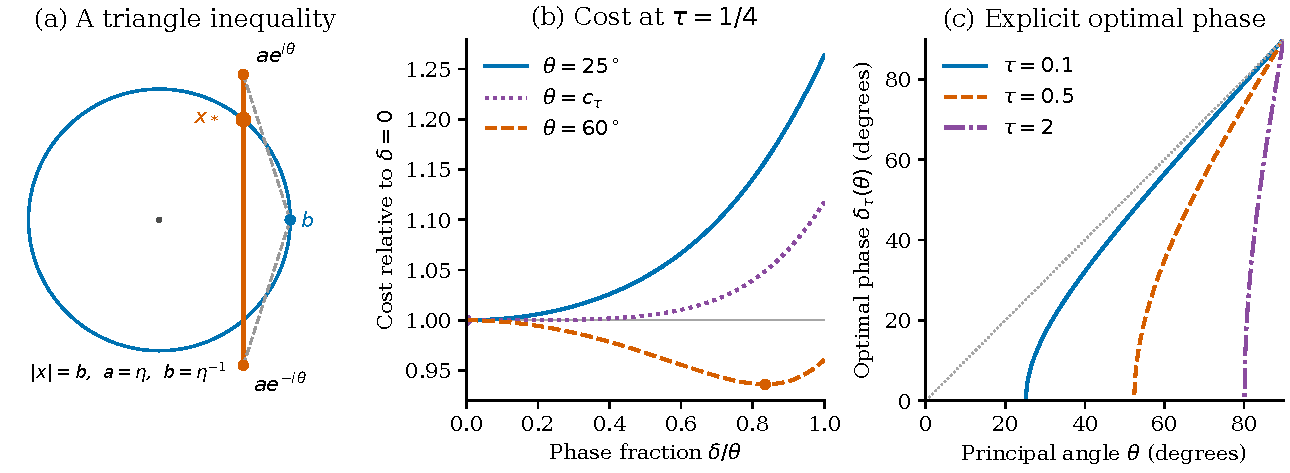
\includegraphics[width=\linewidth]{figures/smoothed_transport_diagram.pdf}
 \caption{The smoothed transport transition. (a) At $\tau=1/4$ and
 $\theta=60^\circ$, a minimizing circle point $x_*$ lies on the segment
 between the two foci; the canonical point $b$ gives a longer broken path.
 (b) The phase cost is shown below, at, and above the cutoff; the dotted
 curve is evaluated at $c_\tau$. (c) The exact optimal phase for three
 smoothing parameters. The global theorem proves that these independent
 scalar choices attain the unrestricted unitary minimum.}
 \label{fig:smoothed-transport}
\end{figure}

\begin{corollary}[Exact convex relaxation]
\label{cor:smoothed-exact-relaxation}
In the cosine--sine coordinates used above,
\[
 \min_{\substack{Z^*Z\leq I\\ZP=PZ}}\|\eta R-\eta^{-1}Z\|_1
 =\min_{\substack{Z^*Z=I\\ZP=PZ}}\|\eta R-\eta^{-1}Z\|_1.
\]
A minimizing contraction is diagonal: on both directions of a principal
plane use $\min\{1,\eta^2\cos\theta\}$, and use one on the fixed
directions. A minimizing unitary is obtained by replacing the two entries
on each supercritical plane by $e^{i\delta_\tau(\theta)}$.
\end{corollary}

\begin{proof}
The preceding trace bound applies to every feasible contraction. The
displayed diagonal contraction attains it: on a supercritical plane
the residual is $\eta\sin\theta$ times the quarter-turn matrix.
The scalar formula supplies the unitary attaining the same value.
\end{proof}

\begin{corollary}[An explicit spectral optimizer]
\label{cor:smoothed-spectral-optimizer}
Let $C=\sqrt{I-(P-Q)^2}$, let $R$ be a completed canonical rotation,
and apply the scalar function $c\mapsto\min\{1,\eta^2c\}$ to $C$:
\[
 B=\min\{I,\eta^2C\},\qquad
 Z=B+i\sqrt{I-B^2},\qquad W=RZ^*.
\]
Then $B$ attains the convex relaxation, $Z$ is unitary and commutes
with $P$, and $W$ attains \cref{eq:smoothed-global-minimum}.
All square roots are positive square roots; the minimum defining $B$
is spectral.
\end{corollary}

\begin{proof}
On a cosine eigenspace of eigenvalue $c=\cos\theta$, the factor $Z$
is the scalar
\[
 \min\{1,\eta^2c\}
   +i\sqrt{1-\min\{1,\eta^2c\}^2}
 =e^{i\delta_\tau(\theta)}.
\]
Thus $Z$ is the attaining phase factor from the preceding proof.
The real part $B$ is the attaining contraction from
\cref{cor:smoothed-exact-relaxation}. Since $C$ commutes with $P$,
so do both spectral factors. The formula for $W$ now gives the
required transport and exact cost.
\end{proof}

\begin{corollary}[A quantitative certificate below the transition]
\label{cor:smoothed-stability}
Suppose every principal angle is at most $\theta_*$, where
$0\leq\theta_*<c_\tau$. For every
unitary transporter $W$, the canonical rotation $R$ satisfies
\[
 \Psi_\tau(W)-\Psi_\tau(R)
 \geq
 \frac{\cos\theta_*-\eta^{-2}}
      {2\sqrt{\tau^2+2-2\cos\theta_*}}\,\|W-R\|_F^2.
\]
Thus an objective error bounds the Frobenius distance from the unique
minimizer, with a constant determined by the largest principal angle.
\end{corollary}

\begin{proof}
Write $W=RZ^*$ as above. Retaining the slack in the dual certificate gives
\[
 \Psi_\tau(W)-\Psi_\tau(R)
 \geq b\sum_\ell h_\ell
       \bigl(1-\operatorname{Re}\langle e_\ell,Ze_\ell\rangle\bigr),
 \qquad
 h_\theta=\frac{a\cos\theta-b}
                  {\sqrt{a^2+b^2-2ab\cos\theta}},
\]
with $h_\ell=1$ on fixed directions. Unitarity gives
$1-\operatorname{Re}\langle e,Ze\rangle=\|(Z-I)e\|^2/2$.
The function $(ac-b)/\sqrt{a^2+b^2-2abc}$ is increasing in $c$:
its derivative is
$a^2(a-bc)/(a^2+b^2-2abc)^{3/2}>0$ for $c\in[b/a,1]$.
Consequently $h_\ell\geq h_{\theta_*}>0$. Sum over the basis, use
$\|Z-I\|_F=\|W-R\|_F$, and substitute $ab=1$ and $b=\eta^{-1}$.
\end{proof}


For a feasible numerical candidate whose objective is at most $\varepsilon$
above the minimum, \cref{cor:smoothed-stability} yields
\[
 \|W-R\|_F\leq
 \left(
 \frac{2\sqrt{\tau^2+2-2\cos\theta_*}}
      {\cos\theta_*-\eta^{-2}}\,\varepsilon
 \right)^{1/2}.
\]
The constant depends on the angle bound and smoothing parameter and is
independent of the ambient dimension. The explicit construction and
support certificate therefore supply an exact benchmark for constrained
numerical optimization, including a distance guarantee in the strict
subcritical regime.

\begin{theorem}[Quartic stability through the transition]
\label{thm:smoothed-quartic-stability}
Suppose every principal angle is at most $c_\tau$ and $n\geq1$.
For every unitary transporter $W$, the canonical rotation satisfies
\[
 \Psi_\tau(W)-\Psi_\tau(R)
 \geq \frac{3\tau}{32\eta^4n}\,\|W-R\|_F^4.
\]
Thus $R$ is the unique minimizer, including when critical and smaller
angles occur together. An objective error at most $\varepsilon\geq0$
implies
\[
 \|W-R\|_F\leq
 \left(\frac{32\eta^4n}{3\tau}\,\varepsilon\right)^{1/4}.
\]
\end{theorem}

\begin{proof}
Write $a=\eta$, $b=\eta^{-1}$, so $a-b=\tau$, and set
$W=RZ^*$ with $ZP=PZ$. Choose $0\leq\delta\leq b$ and use the
nuclear support unitary selected at $\beta=b-\delta$ in place of $b$.
On a principal plane its diagonal weight is
\[
 h_\beta(\theta)=
 \frac{a\cos\theta-\beta}
      {\sqrt{(a\cos\theta-\beta)^2+a^2\sin^2\theta}}
 \geq \frac{\delta}{a}.
\]
Indeed $a\cos\theta\geq b$, while the denominator is at most $a$.
The fixed directions retain weight one.

The change of support introduces a second-order error. For complex
$u\ne0$ and $v$, the identity $(|v|-|u|)^2\geq0$ gives
\[
 |v|-\operatorname{Re}\left(\frac{\bar u}{|u|}v\right)
 \leq \frac{|v-u|^2}{2|u|}.
\]
Apply this with $u=ae^{i\theta}-\beta$ and $v=ae^{i\theta}-b$.
Since $|u|\geq a-\beta\geq\tau$, the total support loss is at most
$n\delta^2/(2\tau)$. Keeping the diagonal defect as in
\cref{cor:smoothed-stability}, and putting $D=\|W-R\|_F$, yields
\[
 \Psi_\tau(W)-\Psi_\tau(R)
 \geq \frac{b\delta}{2a}D^2-\frac{n\delta^2}{2\tau}.
\]
Unitarity gives $D^2\leq4n$. The choice
$\delta=b\tau D^2/(4an)$ therefore lies in $[0,b]$ and makes the
right-hand side $3b^2\tau D^4/(32a^2n)$. Substitute $ab=1$.
\end{proof}

\begin{corollary}[The exact canonical cutoff]
\label{cor:smoothed-canonical-cutoff}
The completed canonical rotation minimizes $\Psi_\tau$ exactly when
$\theta_j\leq c_\tau$ for every principal angle. In that regime it is
the unique minimizer. The global minimum is unique exactly in this regime.
If any principal angle exceeds $c_\tau$, the spectral-phase optimizer in \cref{cor:smoothed-spectral-optimizer} has
strictly lower cost than the canonical rotation. Reversing all its scalar
phases gives a second, distinct global minimizer.
\end{corollary}

\begin{proof}
When all angles are at most the cutoff, the scalar formula selects zero
phase, and \cref{thm:smoothed-quartic-stability} gives uniqueness.
If an angle exceeds the cutoff, the unique scalar minimizing phase on
that plane is positive; replacing its zero phase strictly decreases the
sum. The unrestricted global optimizer attains at most this improved cost.
The scalar cost is even in the phase, so reversing every optimal phase
preserves the attained global value. On a supercritical plane the phase is
in $(0,\pi/2]$, so its two signs give distinct
unitaries. Hence the global minimum is not unique above the cutoff.
\end{proof}

For acute principal angles the cutoff can also be used to choose the
smoothing parameter. The canonical rotation is optimal exactly when
\[
 \tau\geq\frac{1-\cos\theta_j}{\sqrt{\cos\theta_j}}
 \qquad\text{for every }j.
\]
Indeed, writing $x=\sqrt{\cos\theta_j}$ and $b=\eta^{-1}$,
\[
 \tau x-(1-x^2)=(\eta x-1)(1+bx).
\]
The second factor is positive. Thus the smoothing test is equivalent to
$\eta x\geq1$, or $\cos\theta_j\geq\eta^{-2}$.
Increasing the smoothing parameter preserves this condition.

The quadratic estimate gives the stronger local rate when the angle bound
stays strictly below the cutoff. The quartic estimate supplies a nonzero
certificate at equality. The following family admits a sharper constant
and a root bound valid for every objective error.

\begin{proposition}[Stability on a critical isoclinic family]
\label{prop:smoothed-critical-stability}
Let $J$ be a skew-adjoint unitary such that
$(2P-I)J(2P-I)=-J$, and put
\[
 d_\tau=\sqrt{\eta^2-\eta^{-2}},\qquad
 R=\eta^{-2}I+(d_\tau/\eta)J.
\]
Then $R$ rotates the source through the critical angle $c_\tau$ on
every principal plane. For every unitary $W$ with $W(U)=R(U)$,
write $D=\|W-R\|_F$ and $L=nd_\tau$. One has
\[
 \Psi_\tau(W)-\Psi_\tau(R)
 \geq \sqrt{L^2+\frac{D^4}{4\eta^2}}-L.
\]
Consequently an objective error at most $\varepsilon\geq0$ implies
\[
 D^4\leq 4\eta^2\varepsilon(2nd_\tau+\varepsilon).
\]
In particular $R$ is the unique minimizer in this critical family.
\end{proposition}

\begin{proof}
Put $Z=W^*R$; it is unitary and commutes with $P$. Conjugation by
$2P-I$ negates both $J$ and $JZ$, so their traces vanish.
Moreover $\|Z-I\|_F=D$ and
$n-\operatorname{Re}\operatorname{tr}Z=D^2/2$.
For every real $t$, the matrix
$T_t=(\cos t)J+(\sin t)I$ is unitary. Its nuclear support pairing with
$\eta R-\eta^{-1}Z=d_\tau J+\eta^{-1}(I-Z)$ is
\[
 \operatorname{Re}\operatorname{tr}
   \bigl(T_t^*(\eta R-\eta^{-1}Z)\bigr)
 =L\cos t+\frac{D^2}{2\eta}\sin t.
\]
The maximum over $t$ is
$\sqrt{L^2+D^4/(4\eta^2)}$. The canonical weighted nuclear cost is
$L$, proving the first inequality. Squaring after adding $L$ gives the
error estimate, whose zero-error case proves uniqueness.
\end{proof}

\begin{proposition}[Quartic flatness at the cutoff]
\label{prop:smoothed-critical-flatness}
Put $b=\eta^{-1}$ and $d=d_\tau$. For $|z|=1$, define
\[
 G(z)=|b+id-bz|+|b-id-bz|-2d.
\]
If $|b\operatorname{Im}z|\leq d/2$, then
\[
 0\leq G(z)\leq\frac{b^2}{2d}|z-1|^4.
\]
The exact leading coefficient is
\[
 \lim_{\substack{z\to1,\ |z|=1\\z\ne1}}
   \frac{G(z)}{|z-1|^4}=\frac{b^2}{4d}.
\]
For every $c>0$ and $r>0$ there is a unit phase $z$ with
$0<|z-1|<r$ and $G(z)<c|z-1|^2$.
Consequently, on a critical principal plane no positive quadratic growth
constant holds in any neighborhood of the canonical rotation.
\end{proposition}

\begin{proof}
Write $bz=x+iy$, $h=b-x$, $s_-=d-y$ and $s_+=d+y$.
The imaginary-part condition gives $s_\pm\geq d/2$. Since
$\sqrt{h^2+s^2}-s=h^2/(\sqrt{h^2+s^2}+s)$, each focal-distance
excess is at most $h^2/d$. The circle identity gives
$|bz-b|^2=2bh$, so their sum is at most
$2h^2/d=b^2|z-1|^4/(2d)$. Nonnegativity follows from the triangle
inequality between the foci.

The rational circle points
\[
 z(t)=\frac{1-t^2+2it}{1+t^2},\qquad t>0,
 \qquad |z(t)-1|^2=\frac{4t^2}{1+t^2},
\]
approach one through distinct unit phases. The quartic upper bound makes
$G(z(t))/|z(t)-1|^2$ tend to zero, proving the assertion for every
$c,r>0$. For the leading coefficient, rationalize both focal terms:
\[
 G(z)=h^2\left(
 \frac1{\sqrt{h^2+s_-^2}+s_-}
 +\frac1{\sqrt{h^2+s_+^2}+s_+}\right).
\]
Since $h^2=b^2|z-1|^4/4$ and both denominators tend to $2d$,
the displayed limit follows.
On a critical principal plane, $\eta R$ has eigenvalues $b\pm id$.
Unitary invariance and \cref{eq:smoothed-weighted-nuclear} identify
$G(z)$ with $\Psi_\tau(\bar z R)-\Psi_\tau(R)$, while
$\|\bar z R-R\|_F^2=2|z-1|^2$. These scalar phases remain feasible
transporters, so a quadratic estimate would contradict the preceding
assertion. In particular, along these phases the cost excess divided by
$\|\bar z R-R\|_F^4$ tends to $b^2/(16d)$. This is also the leading
coefficient of the root lower bound in
\cref{prop:smoothed-critical-stability} at $n=2$.
\end{proof}

\begin{corollary}[Sharp sensitivity to angle errors]
\label{cor:smoothed-value-sensitivity}
For $\theta,\varphi\in[0,\pi/2]$,
\[
 |\mu_\tau(\theta)-\mu_\tau(\varphi)|
 \leq\frac2\eta|\theta-\varphi|.
\]
The coefficient $2/\eta$ is the least constant valid on this interval.
For two angle lists of the same length, the error in the exact minimum
therefore satisfies
\[
 \left|\sum_j\mu_\tau(\theta_j)-\sum_j\mu_\tau(\varphi_j)\right|
 \leq\frac2\eta\sum_j|\theta_j-\varphi_j|.
\]
\end{corollary}

\begin{proof}
Below the cutoff, put $d(\theta)=\sqrt{\tau^2+2-2\cos\theta}$.
The derivative is $2\sin\theta/d(\theta)$. With $b=\eta^{-1}$,
\[
 b^2d(\theta)^2-\sin^2\theta=(\cos\theta-b^2)^2\geq0,
\]
so its absolute value is at most $2b$. Above the cutoff, the derivative
is $2\eta\cos\theta\leq2b$. The two branches have the same value
and derivative at $c_\tau$; the common derivative there is $2b$.
The mean value theorem gives the bound, and this derivative proves that
the coefficient cannot be decreased. The list estimate follows by the
triangle inequality.
\end{proof}

As $\tau\downarrow0$, the angle cost tends to $2\sin\theta$, recovering
\cref{thm:complex-trace-all-pairs}. As $\tau\to\infty$,
$2\tau\mu_\tau(\theta)$ tends to $8\sin^2(\theta/2)$, the squared
Frobenius displacement of the canonical planar rotation. Thus this family
connects the trace optimum with the classical quadratic minimum while
locating exactly where the optimizing phase changes.

\begin{corollary}[Exact correction to a commuting unitary]
\label{cor:smoothed-commuting-correction}
Let $A$ be unitary and let $P$ project onto $U$. Put $V=A(U)$ and
let $W_*$ be the optimizer in \cref{cor:smoothed-spectral-optimizer}
for $U,V$. Then $C_*=W_*^*A$ commutes with $P$ and minimizes
\[
 \sum_{j=1}^n \rho_\tau(\sigma_j(A-C))
 \quad\text{over unitary }C\text{ with }CP=PC.
\]
Its exact minimum is $\sum_{j=1}^r\mu_\tau(\theta_j)$, where
$\theta_j$ are the principal angles between $U$ and $A(U)$.
\end{corollary}

\begin{proof}
The maps $W\mapsto W^*A$ and $C\mapsto AC^*$ give inverse
bijections between unitary transporters from $U$ to $A(U)$ and
unitaries preserving $U$. A unitary preserves $U$ exactly when it
commutes with $P$. Since $A-C=(W-I)C$ when $W=AC^*$, unitary
invariance identifies the two singular-value costs. Apply
\cref{thm:smoothed-transport,cor:smoothed-spectral-optimizer}.
\end{proof}

When every angle is at most $c_\tau$, this correction is $C_*=R^*A$
and is unique. If a feasible correction $C$ has objective error at most
$\varepsilon\geq0$, then
\[
 \|C-C_*\|_F\leq
 \left(\frac{32\eta^4n}{3\tau}\,\varepsilon\right)^{1/4}.
\]
The quadratic estimate of \cref{cor:smoothed-stability} transfers as well
when the angles stay strictly below the cutoff. Indeed,
$W=AC^*$ satisfies
$\|W-R\|_F=\|C-R^*A\|_F$, and the preceding proof identifies their
objective errors.

Canonical optimality has a direct test in terms of the commutation defect:
\[
 R^*A\text{ is globally optimal}
 \quad\Longleftrightarrow\quad
 \|AP-PA\|\leq\sqrt{1-\eta^{-4}},
\]
where $\|\cdot\|$ is the operator norm. To see this, use
$\|AP-PA\|=\|P-APA^*\|=\max_j\sin\theta_j$, with value zero for an
empty angle list, and apply \cref{cor:smoothed-canonical-cutoff}.
The closest feasible correction is unique exactly when this inequality
holds, including equality. Above it, the opposite phase choices give
distinct minimizing corrections.

This gives an exact correction that preserves both a specified subspace
and its orthogonal complement. The construction requires spectral
functions of the two projections; it provides the value and an optimizer
without an iterative search over the unitary group.

For spectral projections, the correction preserves a selected spectral
subspace and its orthogonal complement while retaining global unitarity.
Constructions of nearby operators commuting with a spectral projection
are established in approximate symmetry theory \citep{chubb2017approximate}; the formula above gives the
exact minimum and an explicit correction for this spectral penalty.
